\documentclass[11pt,a4paper]{article}
\usepackage[margin=1in]{geometry}
\usepackage[T1]{fontenc}
\usepackage{times}
\usepackage{graphicx}
\usepackage{booktabs}
\usepackage{hyperref}
\usepackage{tikz}
\usepackage{microtype}
\usepackage{setspace}

\title{Exploring Regret- and Deprivation-Like Signals in LLMs: : Automated Pipeline and Preliminary Evidence}
\author{Jaeyeong CHOI \\ DGIST EECS \\ \texttt{jaeyeong2022@dgist.ac.kr}}
\date{\today}

\begin{document}
\maketitle

\begin{abstract}
We do not claim that large language models (LLMs) experience emotion.
Instead, we test whether LLMs show text patterns that are behaviorally similar to human regret-like responses to loss and missed opportunities.
This stage focuses on building a reproducible pipeline for literature screening, prompt control, and iterative experiment execution.
\end{abstract}

\section{Introduction}
Humans often express regret through counterfactual language (\textit{if only...}), self-attribution, and repeated reflection on irreversible events.
Prior work suggests that apparent social-emotional behavior in LLMs is sensitive to prompt format, so observed signals should be evaluated as task-dependent behavior rather than internal affect.

\section{Methods}
The study pipeline consists of four steps.
\begin{enumerate}
  \item \textbf{Literature collection and screening:} OpenAlex query + rule-based screening.
  \item \textbf{Prompt bank expansion:} scenario and persona variations for loss, reversal, and reflection.
  \item \textbf{Experiment runner:} scenario/persona/temperature combinations with reproducible metadata logging.
  \item \textbf{State tracking:} continuous status files, scheduled jobs, and compact summaries.
\end{enumerate}

\section{Current Results}
Table~\ref{tab:status} and Figure~\ref{fig:progress} show the current progress.

\begin{table}[t]
\centering
\caption{Current status snapshot}
\label{tab:status}
\begin{tabular}{lccc}
\toprule
\textbf{Item} & \textbf{Value} & \textbf{Interpretation} & \textbf{Status} \\
Literature candidates & 279 & Core review pool before strict curation & Screening in progress \\
Evidence-table rows & 279 & Auto-synced from retrieval log & Stable \\
Validation samples & 109,500 & Mock-data stress tests only & Running \\
Cron interval & 1 minute & Continuous automation & Auto-retrying \\
Overall stage & 52\\\% prepared & Pre-experiment stage & On track \\
\bottomrule
\end{tabular}
\end{table}

\begin{figure}[t]
\centering
\resizebox{0.9\textwidth}{!}{%
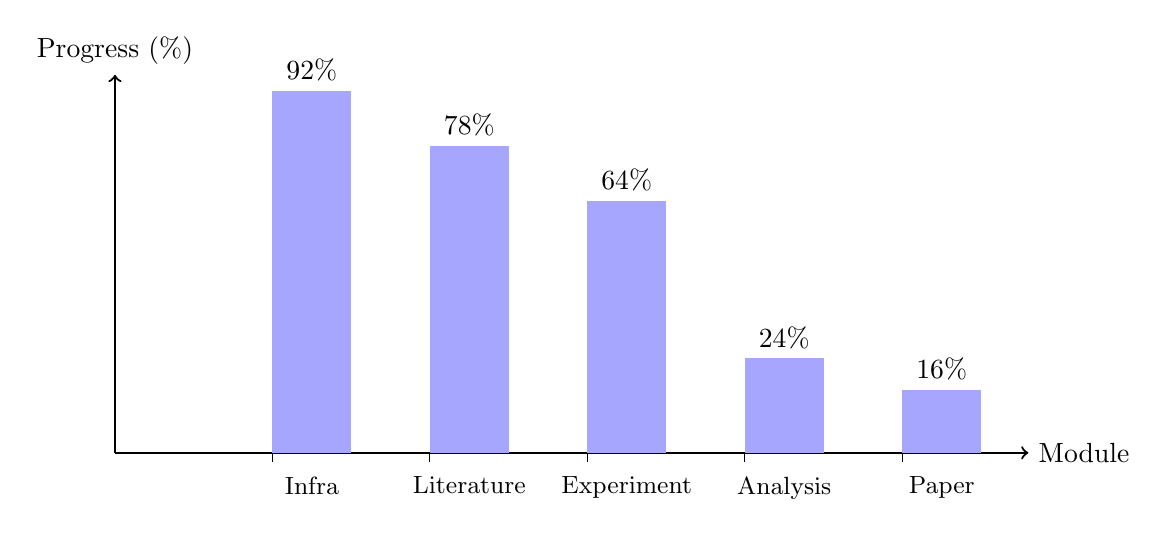
\begin{tikzpicture}[x=2cm,y=1.5cm]
  \draw[->,thick] (0,0) -- (5.8,0) node[right]{Module};
  \draw[->,thick] (0,0) -- (0,3.2) node[above]{Progress (\%)};
  \foreach \x in {1,...,5} {
    \draw (\x,0) -- (\x,-0.08);
  }
  \foreach \x/\lab/\y in {1/Infra/92,2/Literature/78,3/Experiment/64,4/Analysis/24,5/Paper/16} {
    \fill[blue!35] (\x,0) rectangle +(0.5,\y/30);
    \node[below] at (\x+0.25,-0.12) {\small \lab};
    \node[above] at (\x+0.25,\y/30) {\y\%};
  }
\end{tikzpicture}}
\caption{Module-wise progress from the live dashboard. Figure width is constrained to 0.9\\textwidth to prevent overflow.}
\label{fig:progress}
\end{figure}

\section{Discussion}
The infrastructure is now reproducible and automatable.
Next we must move from synthetic-generation checks to real-model calls and run mixed-effects analyses for prompt, persona, and temperature interactions.

\section{Limitations}
Current results are preliminary:
\begin{itemize}
  \item Core evidence relies on mock-generated baseline data.
  \item Literature screening is candidate-level and not yet a fully curated gold set.
  \item Statistical claims are pending full model outputs.
\end{itemize}

\section{Next Steps}
\begin{enumerate}
  \item Run real-model batches (at least 30 samples per condition).
  \item Add interaction modeling and robustness checks.
  \item Add blinded human annotation for interpretability validity.
  \item Convert this report into a final manuscript with full citations and figures.
\end{enumerate}

\section{Conclusion}
This study establishes a reusable, transparent pipeline for evaluating regret-like language behavior claims in LLMs. The next phase is inference-strong testing with production model outputs.

\begin{thebibliography}{99}
\bibitem{kosinski2024tom}
Kosinski, M. (2024). Evaluating large language models in theory of mind tasks.

\bibitem{epstude2008}
Epstude, K. and Roese, N. J. (2008). The functional theory of counterfactual thinking.

\bibitem{roese2017}
Roese, N. J. and Epstude, K. (2017). What have we learned about regret?

\bibitem{ullman2023}
Ullman, T. (2023). Large language models fail on trivial alterations to theory-of-mind tasks.

\bibitem{strachan2024}
Strachan, J. W. A., et al. (2024). Testing theory of mind in large language models and humans.

\bibitem{kim2023}
Kim, M. J. and Lee, S. H. (2023). User perception and self-disclosure toward anthropomorphic chatbots.
\end{thebibliography}

\end{document}
